% \newprob{lq1}{
%     一個物件 O 放在一片透鏡 $L$ 前,成像 I 如圖中所示。\\
%     An object O is placed in front of lens $L$, the image I is shown in the figure below.
%     \begin{figure}[h!]
%         \centering
%         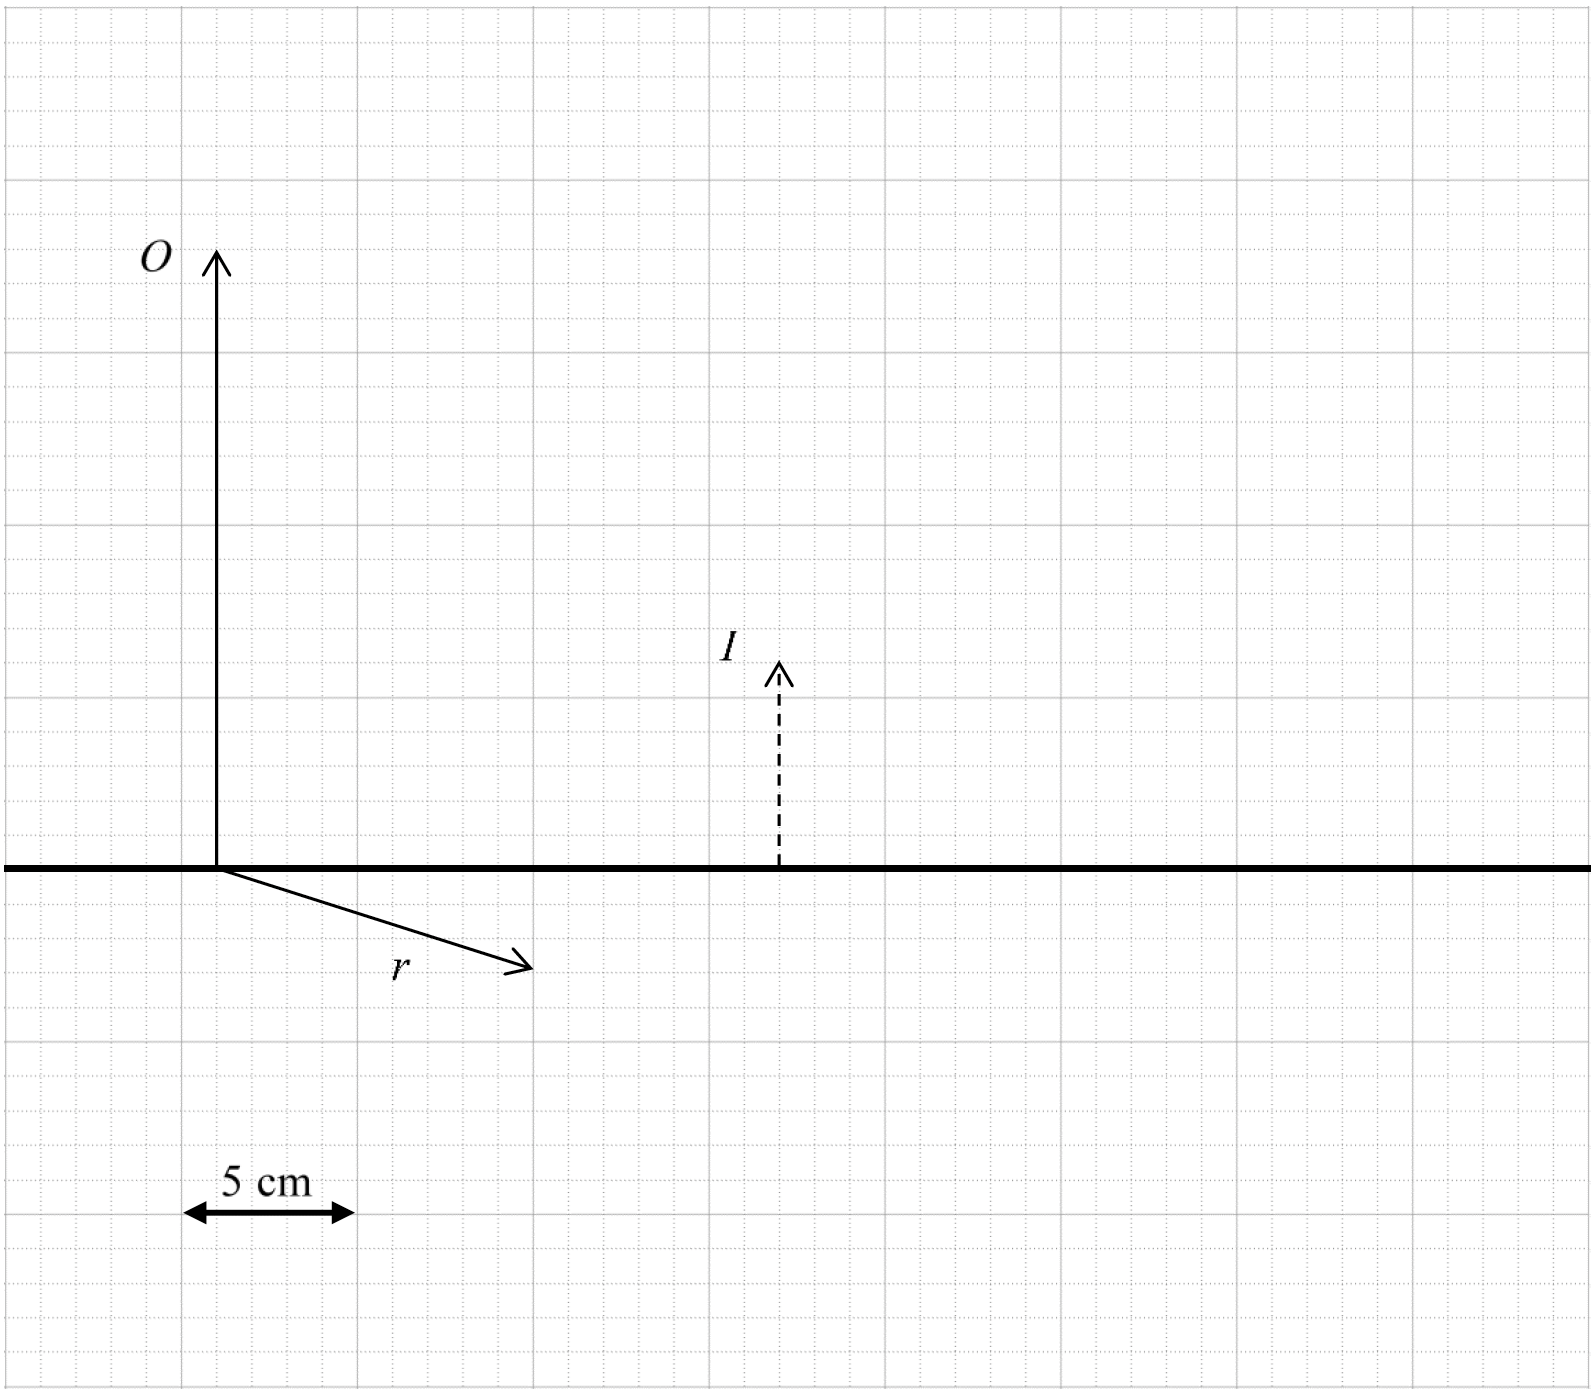
\includegraphics[width=.9\linewidth]{d98n201n20d9d.png}
%     \end{figure}
%     \begin{parts}
%         \part $L$ 是何種透鏡?解釋你的答案。\\
%         what kind of lens is $L$? Explain your answer.\zzh{2}
%         \dlines{2}
%         \clearpage
%         \part 透過加入適當的光線,在圖中畫出透鏡的位置($L$)、主焦點的位置 (F) 並求透鏡焦距。\\
%         By adding suitable ray(s) in the figure, indicate the locations of lens ($L$), principal focus (F) and write down the focal length of the lens.\zzh{5}
%         \vspace{.55cm}\par 焦距focal length: \fillin[][1.5in]

%         \part 完成光線 r 折射後的光路。\\Complete ray r.\zzh{1}
%         \part 透鏡 $L$ 和透鏡 M 的形狀、大小相同,但透鏡 M 的折射率略高。 把透鏡 $L$ 換成透鏡 M 後,成像的放大率會如何改變?扼要解釋你 的答案。\\Lens $L$ and lens M have the same shape and size, but lens M has a slightly higher refractive index. How will the magnification of the image change when lens $L$ is replaced with lens M? Briefly explain your answer.\zzh{2}
%         \dlines{1}
%     \end{parts}
% }{}

\newprob{1716026155}
{
    % active phys p282(266) q11
    一個物體(圖中沒有顯示)置於一塊凹透鏡前, 成像1如圖。符號F'表示透鏡的主焦點。
    \par{\par\centering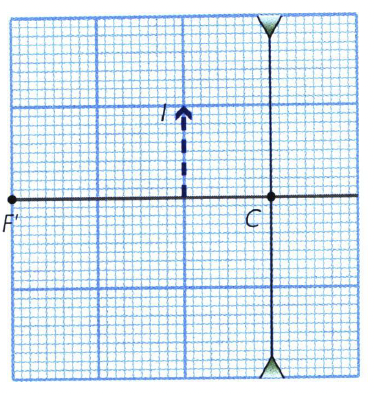
\includegraphics[width=.45\textwidth]{./img/ch3_lens_lq_2024-05-18-17-56-56.png}\par}
    \begin{parts}
        \part 試輔以合適的光線,在圖中標示物體的位置。\zzh{3}
        \part 若像的高度為15 cm,求物體的高度。\zzh{2}
    \end{parts}
}{
    \sol\par{\par\centering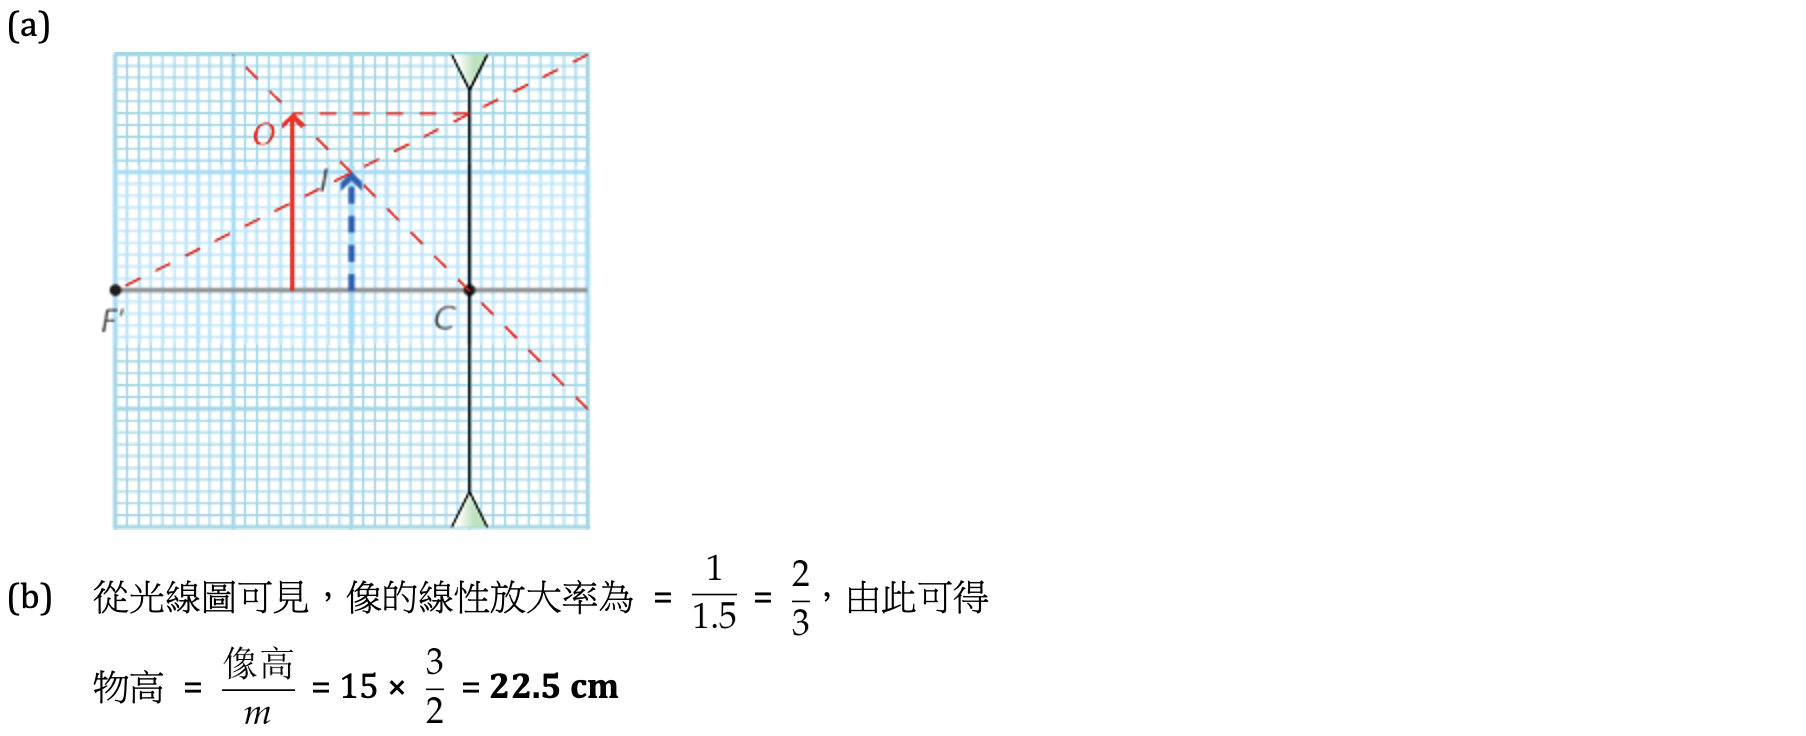
\includegraphics[width=\textwidth]{./img/ch3_lens_lq_2024-05-18-18-00-28.png}\par}
}

\newprob{lq2}{
    把一件高15 cm的物體,放在凸透鏡前45 cm的 位置。下圖顯示兩條從物體發出的光線,及其中 一條折射線。
    % \\An object of height 15 cm is placed 45 cm in front of a convex lens. The figure shows two light rays emitted from that object. One of the paths is as depicted.
    \bigskip\here{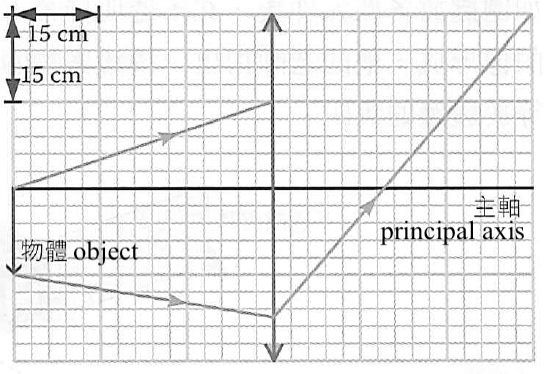
\includegraphics[width=0.6\linewidth]{dwqi0mid9d.png}}\bigskip
    \begin{parts}
        \part 試畫上餘下的折射線。
        % \\Complete the path of the remaining light ray. 
        \zzh{2}
        \part 由此或以其他方法,求透鏡的焦距。
        % \\Hence, or otherwise, find the focal length of the lens. 
        \zzh{1}
        \vspace{.55cm}\par 焦距: \fillin[][1.5in]
        \bigskip
        \part 指出像的本質。
        % \\State the nature of the image, explain your answer.
        \zzh{2}
        \dlines{1}

    \end{parts}
}{
    \sol
    \begin{enumerate}[label=(\alph*)]
        \item \topalign{\par\centering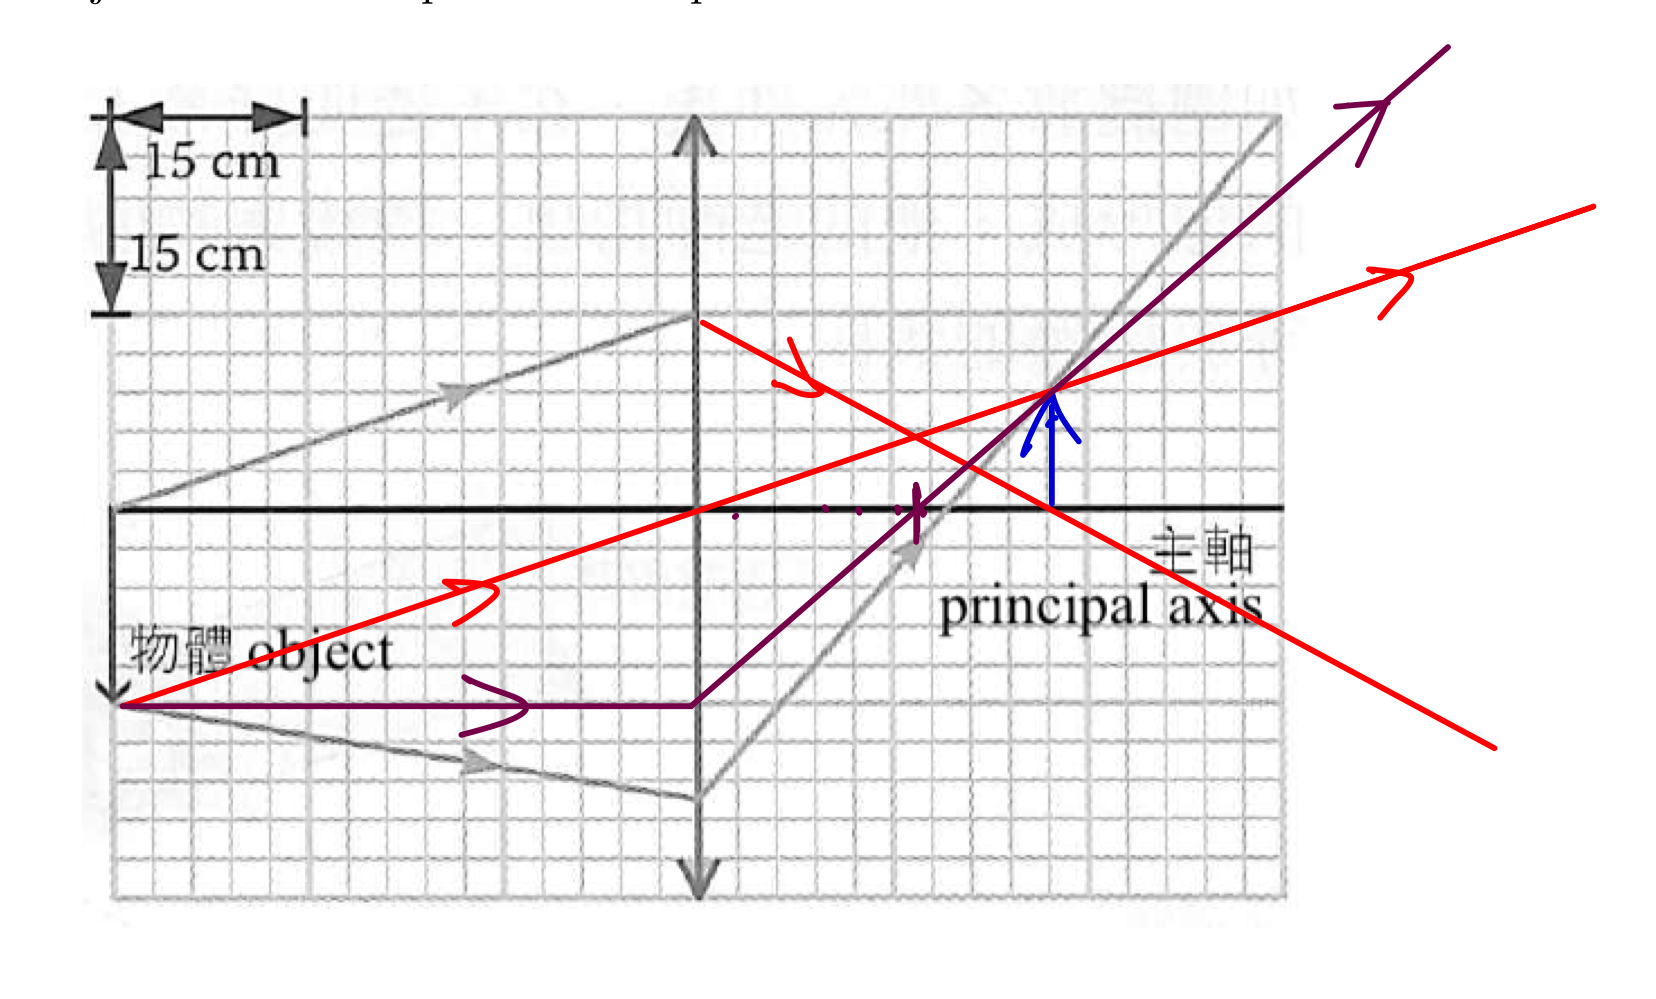
\includegraphics[width=.4\textwidth]{./img/ch3_lens_lq_2024-05-18-20-06-14.png}\par}\giveScore{2}
        \item  焦距=\qty{16.5}{cm}\giveA
        \item 倒置、實像、縮小\giveScore{2}
    \end{enumerate}
}


\newprob{lq3}{
    如圖所示,一位學生用透鏡觀看發光的字母「F」。
    % \\An illuminated letter `F' is viewed through a lens as follow.

    \bigskip{\par\centering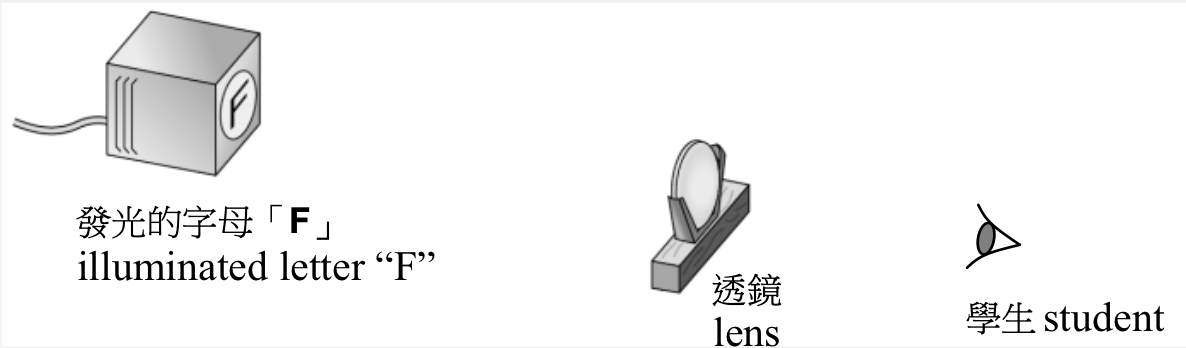
\includegraphics[width=0.7\linewidth]{cdcce.png}\par}\bigskip
    \begin{parts}
        \part 不論透鏡和字母「F」之間的距離怎樣改變,透鏡都不能產生實像。這是哪一種透鏡?
        % \\The lens cannot form a real image of the letter no matter how the distance between them is varied. State the type of lens used.
        \zzh{1}
        % \ddlines{.5}
        \part 草繪學生看到的像。
        % \\Sketch the image as seen by the observer.
        \zzh{1}
        \bigskip\here{
            
\includegraphics[width=0.2\linewidth]{9j290c3c0e92.png}
        }
        % \clearpage
        \part 透鏡的焦距是 15 cm,形成的像與透鏡相距 10 cm。在下面的方格紙中繪畫光線圖,顯示像怎樣形成。
        % \\The focal length of the lens is 15 cm and the image formed is 10 cm away from the lens. In the following graph paper, draw a ray diagram to show how the image is formed.
        \zzh{3}
        {\par
            \centering
            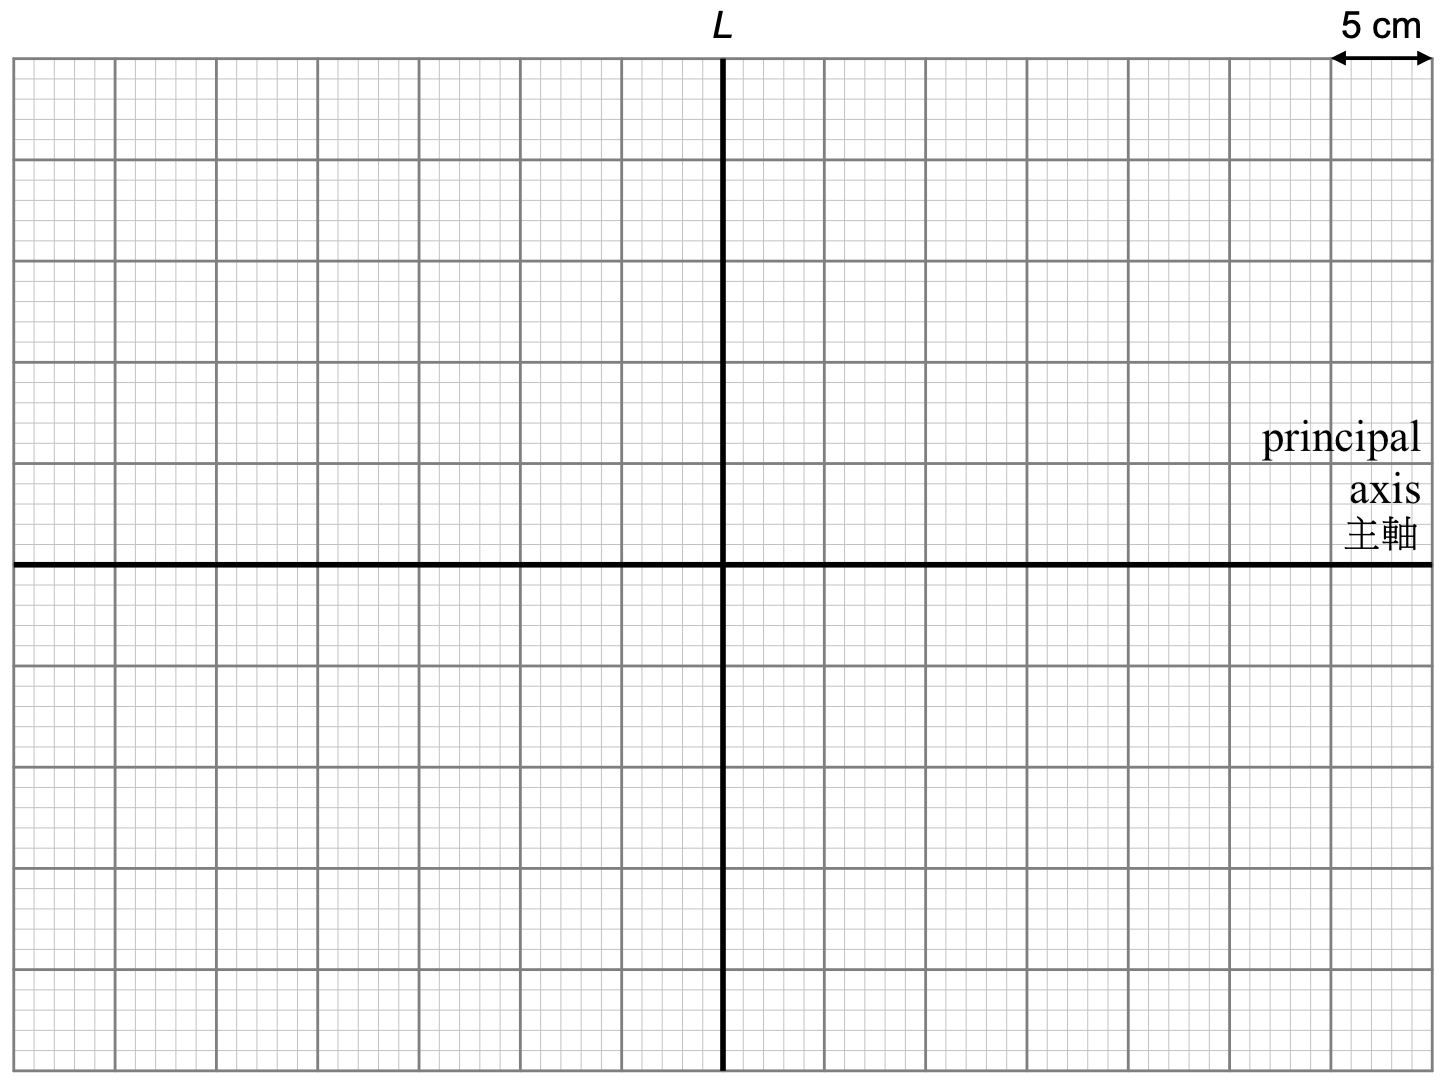
\includegraphics[width=0.75\linewidth]{d8un293u1d3.png}
            \par}
        \part 如果學生把透鏡移近字母「F」,像距、像的方向和線性放大率會怎樣改變?
        % \\If the lens is moved closer to the letter ‘F’, how will the image distance, the orientation and of the image change?
        \zzh{3}
        % \dlines{2}
    \end{parts}
}
{
    \begin{figure}
        \centering
        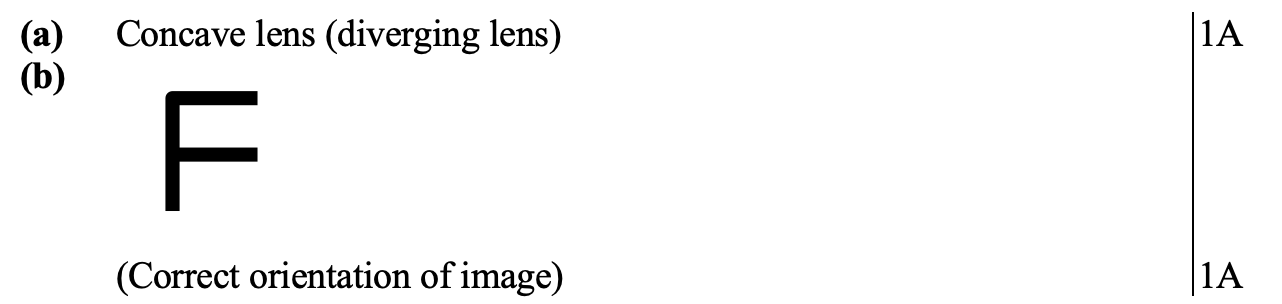
\includegraphics[width=1\linewidth]{dnu28923u8d3.png}
    \end{figure}
    \begin{figure}
        \centering
        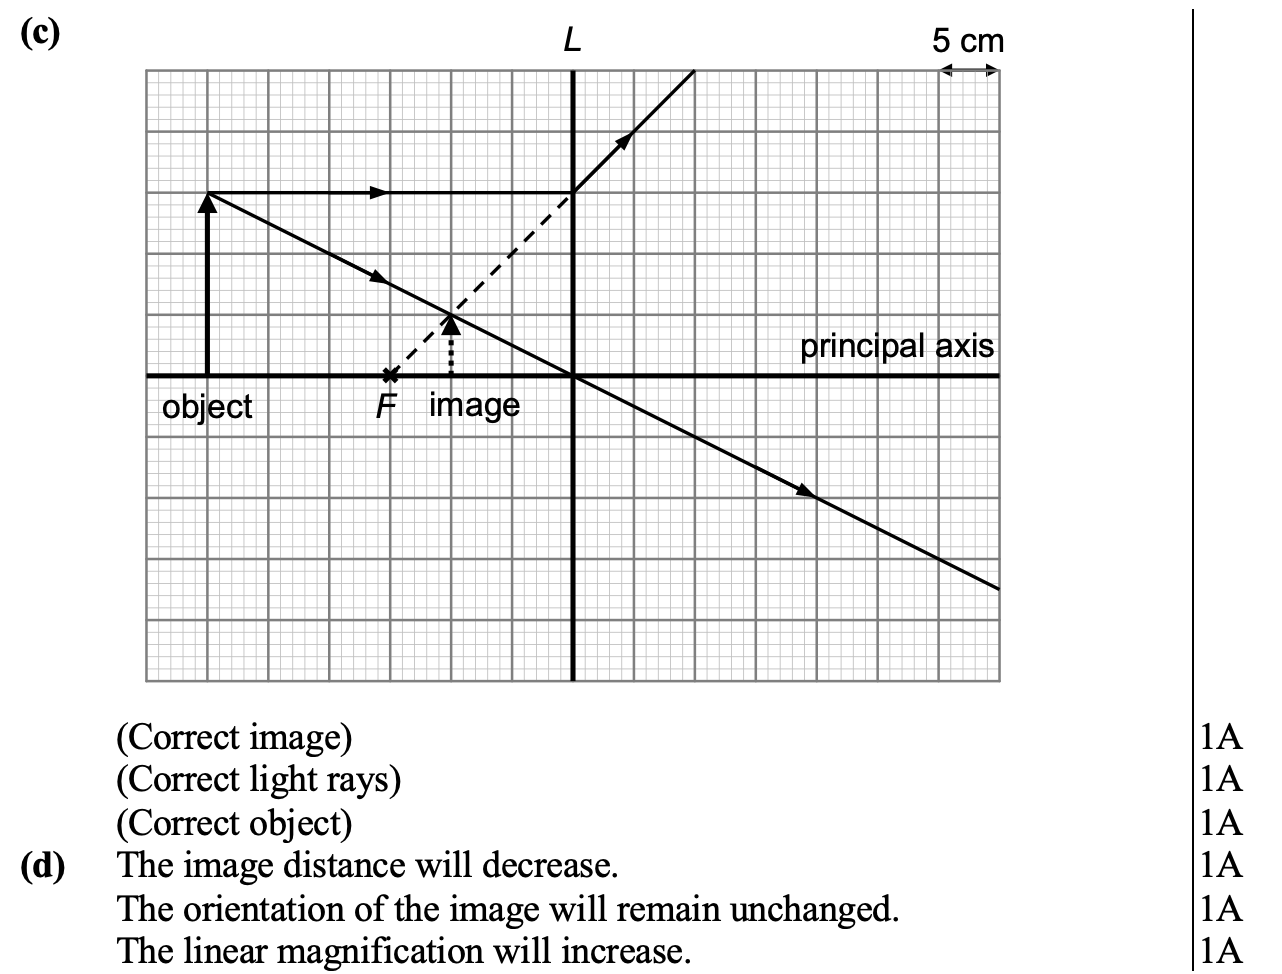
\includegraphics[width=1\linewidth]{92nu0cu2982.png}
    \end{figure}
}


% \newprob{1716025983}
% {
%     % active phys p297(281) q17
%     一個物體高10 cm,置於一 塊凸透鏡前20 cm。在透鏡 另一側60 cm外,放了一塊 屏幕,並能捕捉得到一個清 晰的成像。
%     \par{\par\centering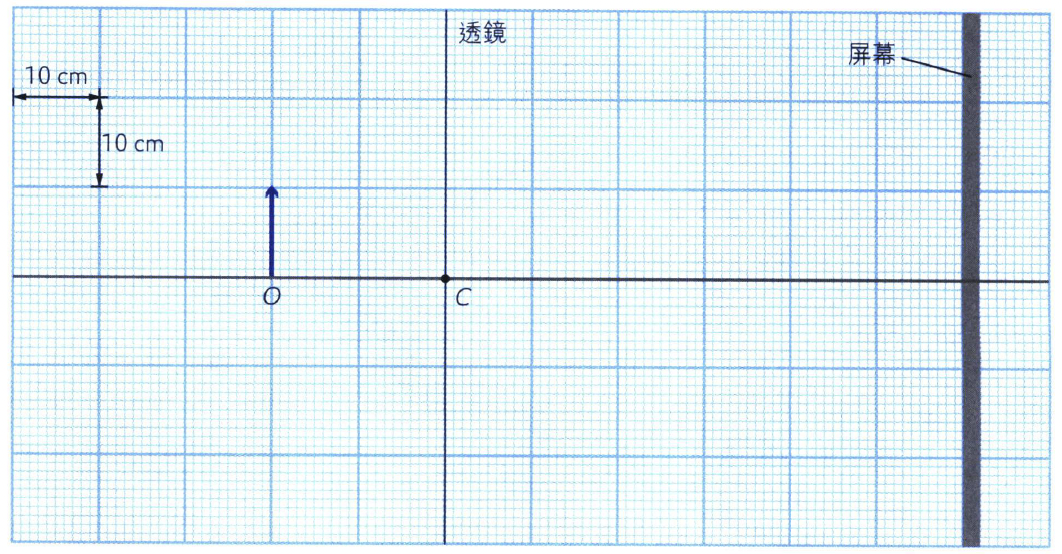
\includegraphics[width=.8\textwidth]{./img/ch3_lens_lq_2024-05-18-17-53-38.png}\par}
%     \begin{parts}
%         \part 所用的透鏡是哪一種?為什麼?\zzh{1}
%         \part 
%         \begin{subparts}
%             \subpart 試繪畫光線圖,表示透鏡如何成像。\zzh{2}
%             \subpart 求透鏡的焦距。\zzh{1}
%         \end{subparts}
%         \part 以一塊中央較厚的透鏡重複實驗。若要捕捉 得到清晰的成像,屏幕應移向何方?\zzh{1}
%     \end{parts}
% }{}